% =====================================================================
% supplementary.tex  --  MOKG-HGNN Supplementary Material
%
% Standalone companion document. Lives in the Zenodo release with the code
% (NOT uploaded to the J-BHI portal, which would count in the 8 pages); cited
% from the main as ~\cite{}. STATO: BOZZA COMPLETA IN PROSA.
%
% Strategia di presentazione: NON un dump di tabelle isolate (una per pagina),
% ma un documento a SEZIONI TEMATICHE. Ogni sezione = breve prosa di contesto
% + la/le sua/e tabella/e; tabelle piccole AFFIANCATE (minipage); font
% leggibili; niente \clearpage gratuiti. Il main le referenzia come testo
% (es. "Table~S2"), quindi ogni rimozione qui va riflessa la'.
%   S1 per-class (assorbe la legenda) · S2 collapse · S3 mechanisms ·
%   Fig.S1 grafo semantico.
% Ablation completa, iperparametri per backbone e template del grafo sono
% stati PROMOSSI nel main (erano S3/S5/S6): non duplicarli qui.
% =====================================================================
\documentclass[10pt]{article}
\usepackage[a4paper,margin=1.9cm]{geometry}
\usepackage{booktabs}
\usepackage{array}
\usepackage{multirow}
\usepackage{graphicx}
\usepackage{amsmath}
\usepackage{amssymb}
\usepackage{caption}
\usepackage{url}

\captionsetup{font=small,labelfont=bf}
\renewcommand{\thetable}{S\arabic{table}}
\renewcommand{\thefigure}{S\arabic{figure}}
\renewcommand{\arraystretch}{1.15}
\setcounter{table}{0}
\setcounter{figure}{0}

\title{\vspace{-1.2em}Supplementary Material\\[0.2em]
\large MOKG-HGNN: A Multi-Scale Heterogeneous Graph Neural Network
Integrating a Biomedical Knowledge Graph for Pan-Cancer Subtype
Classification}
\author{}
\date{}

\begin{document}
\maketitle
\vspace{-2.2em}

\noindent Released with the code on Zenodo and cited from the main text as
Tables~S1--S3 and Fig.~S1. iCluster labels are C1--C28; C24 (LAML) is absent.

\begin{table}[h]
\centering
\caption{Per-class test performance (mean, s.d.\ for F1 in parentheses;
5 seeds). P and R are MOKG-HGNN's; F1 is given for MOKG-HGNN and for the
MOGNN-TF baseline (GCN, 11 seeds) with their difference $\Delta$; $n$ is the
test-set support. Doubles as the iCluster subtype legend.}
\label{tab:s_per_class}
\small
\setlength{\tabcolsep}{5pt}
\begin{tabular}{llr ccc c c}
\toprule
 & & & \multicolumn{3}{c}{\textbf{MOKG-HGNN}} & \textbf{MOGNN-TF} & \\
\cmidrule(lr){4-6}
\textbf{Code} & \textbf{Tumour} & \textbf{$n$} & \textbf{P} & \textbf{R} & \textbf{F1} & \textbf{F1} & \textbf{$\Delta$F1} \\
\midrule
C1 & STAD & 10 & 0.663 & 0.560 & 0.576\,(0.120) & 0.709\,(0.142) & $-0.133$ \\
C2 & BRCA & 30 & 0.542 & 0.680 & 0.602\,(0.021) & 0.737\,(0.077) & $-0.135$ \\
C3 & SARC & 91 & 0.771 & 0.765 & 0.767\,(0.047) & 0.818\,(0.039) & $-0.051$ \\
C4 & COAD & 88 & 0.904 & 0.877 & 0.890\,(0.011) & 0.906\,(0.027) & $-0.016$ \\
C5 & CNS/endocrine & 53 & 0.768 & 0.785 & 0.775\,(0.042) & 0.803\,(0.040) & $-0.028$ \\
C6 & OV & 55 & 0.934 & 0.975 & 0.954\,(0.024) & 0.952\,(0.026) & $+0.002$ \\
C7 & SARC & 39 & 0.221 & 0.308 & 0.257\,(0.031) & 0.262\,(0.068) & $-0.005$ \\
C8 & UCEC & 91 & 0.870 & 0.822 & 0.845\,(0.031) & 0.890\,(0.025) & $-0.045$ \\
C9 & ACC & 27 & 0.893 & 0.948 & 0.917\,(0.026) & 0.904\,(0.027) & $+0.013$ \\
C10 & LUSC & 125 & 0.611 & 0.450 & 0.516\,(0.053) & 0.691\,(0.029) & $-0.174$ \\
C11 & LGG & 81 & 0.953 & 0.943 & 0.948\,(0.010) & 0.973\,(0.015) & $-0.025$ \\
C12 & THCA & 100 & 0.980 & 0.976 & 0.978\,(0.020) & 0.982\,(0.008) & $-0.004$ \\
C13 & mixed (chr8 del) & 42 & 0.332 & 0.467 & 0.387\,(0.063) & 0.458\,(0.070) & $-0.071$ \\
C14 & LUAD & 91 & 0.756 & 0.754 & 0.754\,(0.040) & 0.798\,(0.024) & $-0.044$ \\
C15 & SKCM & 61 & 0.813 & 0.866 & 0.838\,(0.035) & 0.852\,(0.015) & $-0.014$ \\
C16 & PRAD & 95 & 0.994 & 0.975 & 0.984\,(0.016) & 0.991\,(0.006) & $-0.007$ \\
C17 & mixed & 37 & 0.296 & 0.373 & 0.328\,(0.049) & 0.491\,(0.080) & $-0.163$ \\
C18 & pan-GI (MSI) & 57 & 0.545 & 0.761 & 0.634\,(0.041) & 0.769\,(0.060) & $-0.135$ \\
C19 & BRCA & 111 & 0.834 & 0.789 & 0.810\,(0.028) & 0.841\,(0.032) & $-0.031$ \\
C20 & mixed (stromal/immune) & 152 & 0.760 & 0.512 & 0.611\,(0.041) & 0.740\,(0.031) & $-0.129$ \\
C21 & DLBC & 6 & 0.663 & 0.900 & 0.752\,(0.087) & 0.799\,(0.084) & $-0.047$ \\
C22 & SARC & 37 & 0.717 & 0.735 & 0.723\,(0.034) & 0.775\,(0.036) & $-0.052$ \\
C23 & GBM & 10 & 0.665 & 0.860 & 0.745\,(0.075) & 0.696\,(0.061) & $+0.049$ \\
C25 & pan-SCC (chr11 amp) & 56 & 0.433 & 0.529 & 0.473\,(0.082) & 0.783\,(0.054) & $-0.310$ \\
C26 & LIHC & 65 & 0.911 & 0.997 & 0.952\,(0.010) & 0.971\,(0.021) & $-0.019$ \\
C27 & CESC & 114 & 0.769 & 0.719 & 0.743\,(0.034) & 0.809\,(0.027) & $-0.066$ \\
C28 & KIRC & 147 & 0.983 & 0.965 & 0.974\,(0.010) & 0.975\,(0.011) & $-0.001$ \\
\bottomrule
\end{tabular}
\end{table}

\begin{table}[h]
\centering
\caption{Feature collapse, full grid. Test macro-F1 and accuracy (mean, s.d.;
5 seeds) at each gene level, both models on the identical surviving molecular
panel.}
\label{tab:s_collapse}
\small
\setlength{\tabcolsep}{7pt}
\begin{tabular}{llcccc}
\toprule
\textbf{Model} & \textbf{Genes} & \textbf{F1 Macro} & \textbf{s.d.} & \textbf{Acc.} & \textbf{s.d.} \\
\midrule
\multirow{7}{*}{MOKG-HGNN}
 & 700 & 0.7243 & 0.0106 & 0.7570 & 0.0147 \\
 & 500 & \textbf{0.7527} & 0.0044 & 0.7877 & 0.0093 \\
 & 300 & 0.7161 & 0.0062 & 0.7552 & 0.0041 \\
 & 150 & 0.7013 & 0.0092 & 0.7395 & 0.0149 \\
 & 100 & 0.7078 & 0.0092 & 0.7397 & 0.0055 \\
 & 50  & 0.6949 & 0.0095 & 0.7348 & 0.0060 \\
 & 20  & 0.6569 & 0.0123 & 0.6976 & 0.0104 \\
\midrule
\multirow{7}{*}{MOGNN-TF}
 & 700 & \textbf{0.7963} & 0.0099 & 0.8285 & 0.0070 \\
 & 500 & 0.7926 & 0.0212 & 0.8270 & 0.0115 \\
 & 300 & 0.7728 & 0.0084 & 0.8061 & 0.0054 \\
 & 150 & 0.7557 & 0.0076 & 0.7933 & 0.0066 \\
 & 100 & 0.7340 & 0.0132 & 0.7804 & 0.0067 \\
 & 50  & 0.7119 & 0.0200 & 0.7640 & 0.0128 \\
 & 20  & 0.6386 & 0.0246 & 0.7252 & 0.0113 \\
\bottomrule
\end{tabular}
\end{table}

\begin{table}[h]
\centering
\caption{Rank-1 distinctive mechanism per iCluster subtype (pathway and GO
term), from GNNExplainer edge masks with degree normalisation. Names are
truncated for width; full top-15 lists with distinctive scores are released
with the code.}
\label{tab:s_mechanisms}
\footnotesize
\setlength{\tabcolsep}{5pt}
\begin{tabular}{p{1.65cm} p{6.7cm} p{5.85cm}}
\toprule
\textbf{Subtype} & \textbf{Top pathway (rank-1)} & \textbf{Top GO term (rank-1)} \\
\midrule
C1/STAD & Transport of nucleosides and free purine an\,\ldots & muscle contraction \\
C2/BRCA & Tie2 Signaling & transition metal ion binding \\
C3/SARC & Fibronectin matrix formation & metanephric nephron tubule for\,\ldots \\
C4/COAD & Detoxification of Reactive Oxygen Species & methyl-CpG binding \\
C5 & Voltage gated Potassium channels & regulation of blood pressure \\
C6/OV & NGF-independant TRKA activation & metanephric epithelium develo\,\ldots \\
C7/SARC & Synthesis of 15-eicosatetraenoic acid deriv\,\ldots & artery smooth muscle contract\,\ldots \\
C8/UCEC & Estrogen biosynthesis & sex differentiation \\
C9/ACC & RAB geranylgeranylation & glial cell differentiation \\
C10/LUSC & Deactivation of the beta-catenin transacti\,\ldots & transition metal ion binding \\
C11/LGG & DNA Damage/Telomere Stress Induced Senesce\,\ldots & ionotropic glutamate receptor\,\ldots \\
C12/THCA & Prolactin receptor signaling & leukotriene metabolic process \\
C13 & Inositol transporters & liver regeneration \\
C14/LUAD & Defective SFTPA2 causes IPF & multivesicular body lumen \\
C15/SKCM & Methylation & vasodilation \\
C16/PRAD & Activated PKN1 stimulates transcription of\,\ldots & regulation of systemic arteri\,\ldots \\
C17 & Latent infection -- Other responses of Mtb\,\ldots & prostate epithelial cord arbo\,\ldots \\
C18 & Transport of nucleosides and free purine an\,\ldots & electron transport chain \\
C19/BRCA & Growth hormone receptor signaling & blood coagulation, fibrin clot\,\ldots \\
C20 & Chromatin modifying enzymes & intestinal epithelial cell dif\,\ldots \\
C21/DLBC & Insulin processing & circadian rhythm \\
C22/SARC & Cellular Senescence & regulation of AMPA receptor ac\,\ldots \\
C23/GBM & Insulin processing & photoreceptor cell maintenance \\
C25 & Abacavir metabolism & carboxylic acid binding \\
C26/LIHC & Terminal pathway of complement & phospholipid efflux \\
C27/CESC & Activation of BAD and translocation to mito\,\ldots & flavone metabolic process \\
C28/KIRC & Conjugation of phenylacetate with glutamine & fatty acid biosynthetic proce\,\ldots \\
\bottomrule
\end{tabular}
\end{table}

\begin{figure}[h]
\centering
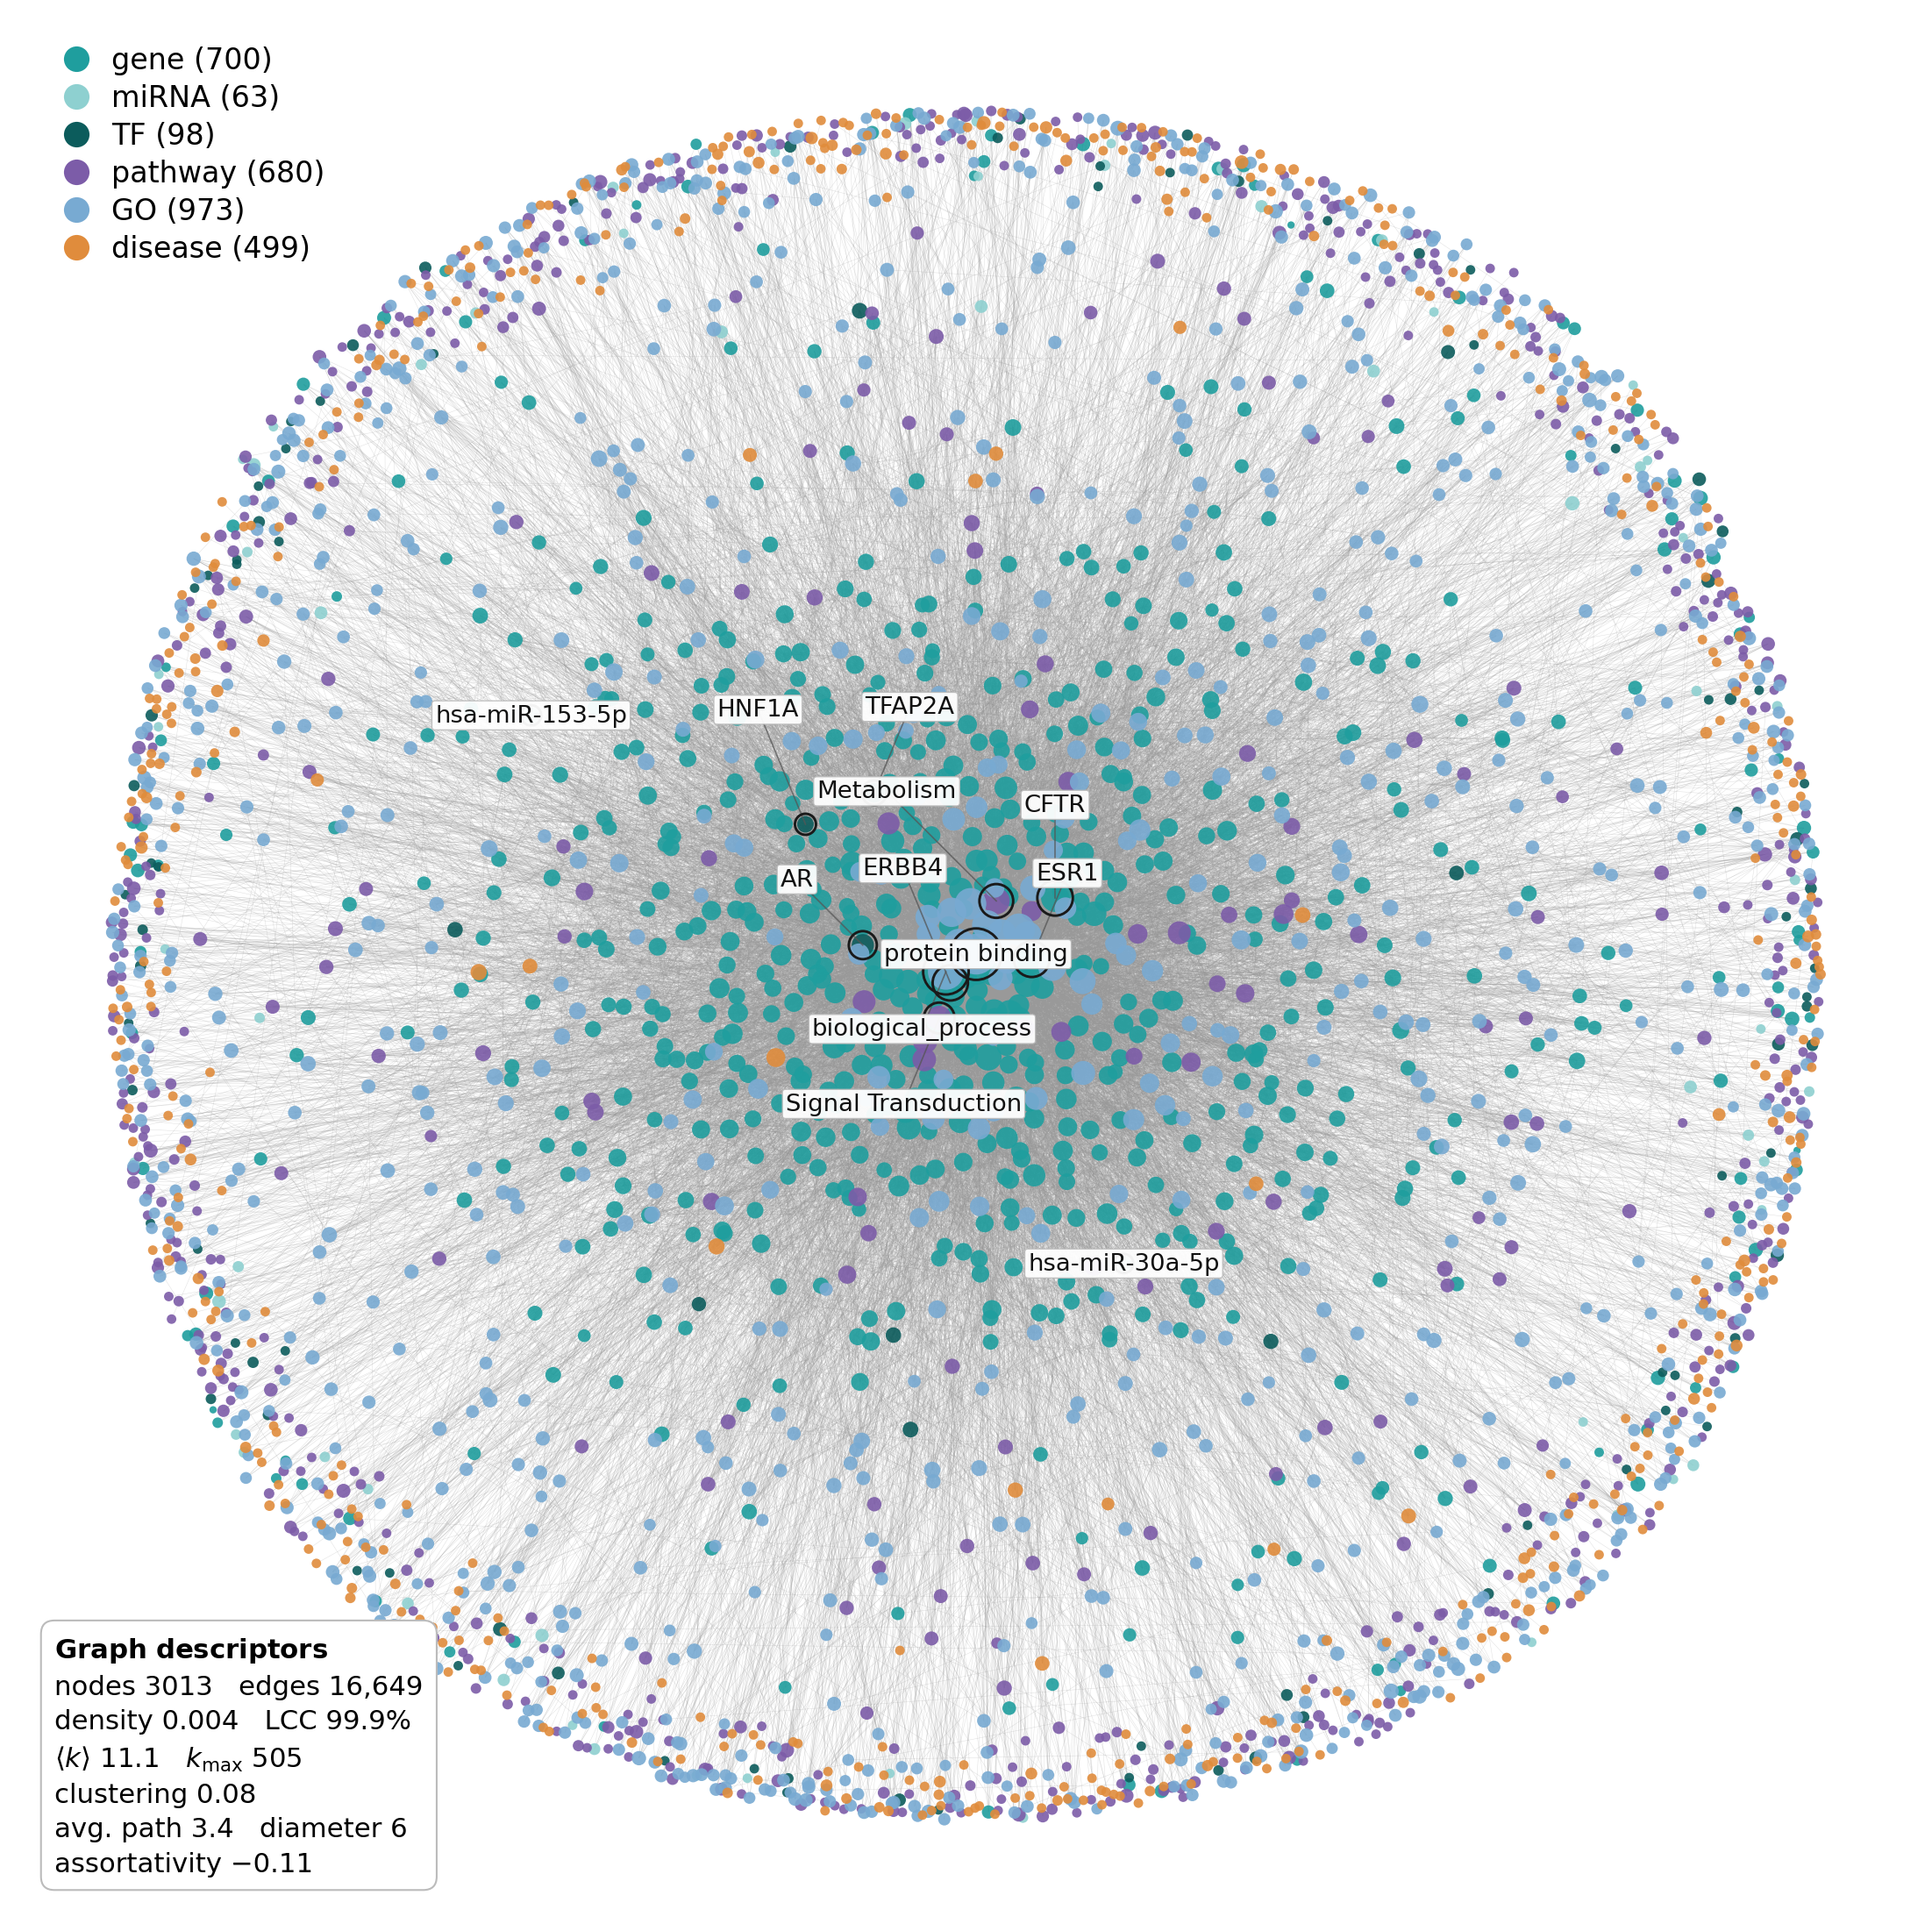
\includegraphics[width=0.86\linewidth]{images/semantic_graph.png}
\caption{The multi-scale template after feature selection, the actual graph
the model operates on. Nodes are the 3013 survivors across six biological
scales (colour); node size is proportional to degree; only the highest-degree
hub of each scale is labelled. Edges are the seven canonical relations
tabulated in the main text; the layout is force-directed
(Fruchterman--Reingold).}
\label{fig:s_graph}
\end{figure}

% =====================================================================
\section*{Reproducibility}
Pipeline (conda env \texttt{gnn}: Python 3.10, PyTorch 2.7 + PyG 2.7, CUDA 12.8):

\begin{quote}\ttfamily\small
setup\_env.sh\\
prepare\_data.sh\hfill\# download KG + TCGA, preprocess\\
make\_graph.sh\hfill\# feature selection + build template\\
train\_and\_eval.sh\hfill\# multi-seed training + evaluation\\
experiments.sh \{per\_class $\vert$ explain\}\\
run\_feature\_collapse.sh\hfill\# MODELS="mokghgnn mognntf"
\end{quote}

\end{document}
